\documentclass[12p]{article}

\usepackage{geometry} % Required to change the page size to A4
\geometry{a4paper} % Set the page size to be A4 as opposed to the default US Letter

\usepackage[utf8]{inputenc}
\usepackage{graphicx}
\usepackage{float} % Allows putting an [H] in \begin{figure} to specify the exact location of the figure
\usepackage{wrapfig} % Allows in-line images such as the example fish picture
\usepackage[nopar]{lipsum} % Used for inserting dummy 'Lorem ipsum' text into the template
\usepackage{fancyhdr}
\usepackage[parfill]{parskip} % Makes sure to put line breaks in between paragraphs and have no indentation
\usepackage{dirtytalk} % Used for quotations (\say{quote})
\usepackage[toc,page]{appendix}
\usepackage{caption}
\usepackage{subcaption}
\usepackage{url}
\usepackage{minted} % Used for including code with syntax highlighting: https://www.sharelatex.com/learn/Code_Highlighting_with_minted

\usepackage[
    style=numeric,
    sorting=none
    ]{biblatex}
\addbibresource{references.bib}

\linespread{1.2} % Line spacing
\setlength\parindent{0pt} % Globally suppress indentation
 
\graphicspath{{pics/}} % Specifies the directory where pictures are stored

\pagestyle{fancy} % Use this, if a header on each page with the section title and page number is wanted
\fancyhf{} % Removes all headers and footers, comment this to show page number at the bottom of each page again
\fancyhead[L]{\rightmark} % Sets the section title on the left side of the header
\fancyhead[R]{\thepage} % Sets the page number on the right side of the header

\newcommand{\HRule}{\rule{\linewidth}{0.5mm}} % Defines a new command for horizontal lines
\newcommand{\SlimHRule}{\rule{\linewidth}{0.25mm}} % Defines a new command for horizontal lines

%----------------------------------------------------------------------------------------

\begin{document}

%----------------------------------------------------------------------------------------
%	TITLE PAGE
%----------------------------------------------------------------------------------------

\begin{titlepage}
    
    \center
    
    %------------------------------------------------
	%	Logo
	%------------------------------------------------
	
	
\includegraphics[width=0.2\textwidth]{pics/AAU_Logo.png}\\[1cm]
    
    %------------------------------------------------
	%	Headings
	%------------------------------------------------
	
	\textsc{\LARGE Aalborg University Copenhagen}\\[1.5cm]
	
	\textsc{\Large P1 Project}\\[0.5cm]
	
	\textsc{\large Group 007}\\[0.5cm]
	
	\textsc{\large IT, Communication and New Media}\\[0.5cm]
	
	
	%------------------------------------------------
	%	Title
	%------------------------------------------------
	
	\HRule\\[0.4cm]
	
	{\huge\bfseries Gangster Squirrel}\\[0.4cm]

	\HRule\\[1.5cm]
	
	%------------------------------------------------
	%	Author(s) and Supervisor(s)
	%------------------------------------------------
	
	\begin{minipage}{0.4\textwidth}
    \begin{flushleft} \large
    \emph{Authors}\\
        Ludvig Alexander \textsc{Brüchmann} \\
        Muheb \textsc{Khan} \\
    	Rehan \textsc{Mir} \\
    	Johannes \textsc{Mols} \\
    	Martin \textsc{Sander} \\
    	Agata \textsc{Surmacz} \\
    	Boris \textsc{Yordanov} \\
    \end{flushleft}
    \end{minipage}
    ~
    \begin{minipage}{0.4\textwidth}
    \begin{flushright} \large
    \emph{Study Numbers} \\
        20174692 \\
        - \\
        20174693 \\
        20174921 \\
        - \\
        20173800 \\
        - \\
    \end{flushright}
    \end{minipage}\\[0.5cm]
    
    %------------------------------------------------
    
    \begin{minipage}{0.4\textwidth}
    \begin{flushleft} \large
    \emph{Supervisors}\\
        Morten \textsc{Falch} \\
        Lene Tolstrup \textsc{Sørensen} \\
    \end{flushleft}
    \end{minipage}
    ~
    \begin{minipage}{0.4\textwidth}
    \begin{flushright} \large
    \end{flushright}
    \end{minipage}\\[0.5cm]

	%------------------------------------------------
	%	Date
	%------------------------------------------------
	
	\vfill\vfill\vfill % Position the date 3/4 down the remaining page
	
	{\large\today} % Date, change the \today to a set date if you want to be precise
	
    
\end{titlepage}

%----------------------------------------------------------------------------------------
%	SYNOPSIS / ABSTRACT
%----------------------------------------------------------------------------------------

\begin{abstract}
\thispagestyle{plain} %Sets the page style for this specific page to plain, to remove the header and show the page number at the bottom
    This is our Abstract, my dudes.

\end{abstract}

\newpage

%----------------------------------------------------------------------------------------
%	TABLE OF CONTENTS
%----------------------------------------------------------------------------------------

\tableofcontents % Include a table of contents
\thispagestyle{plain} %Sets the page style for this specific page to plain, to remove the header and show the page number at the bottom

\newpage % Begins the essay on a new page instead of on the same page as the table of contents 

%----------------------------------------------------------------------------------------
%	INTRODUCTION
%----------------------------------------------------------------------------------------

\section{Introduction}

Text

\begin{center}
    \vspace{1em}
    \SlimHRule\\[0.1cm]
    \Large{Problem formulation}
    \SlimHRule\\[0.1cm]
    \vspace{1em}
\end{center}

Text \medskip

Text

%----------------------------------------------------------------------------------------
%	METHODOLOGY
%----------------------------------------------------------------------------------------

\newpage
\section{Methodology} \label{Methodology}

%----------------------------------------------------------------------------------------
%	STATE OF THE ART
%----------------------------------------------------------------------------------------

\newpage
\section{State of the art}

In this section we have been looking for inspirations for our project. We have identified many of other games that are congruous to what we wanted to do.
We were looking for our competitiors via Google and also we knew a few of them from our own experiences. We have found plenty examples in the Internet and we chose the ones that are, in our opinion, the most similar and related to our game idea. Through this research we wanted to get an overview of general features that this type of games have. Then we will discuss which of them are the most relevant and decide which we would like to implement. This section also helped us to understand the market that we are working in and find out which Ocean Strategy we should use.

%------------------------------------------------

\subsection{Tallowmere} \label{StateOfTheArt_Tallowmere}

\begin{figure}[ht]
    \center
    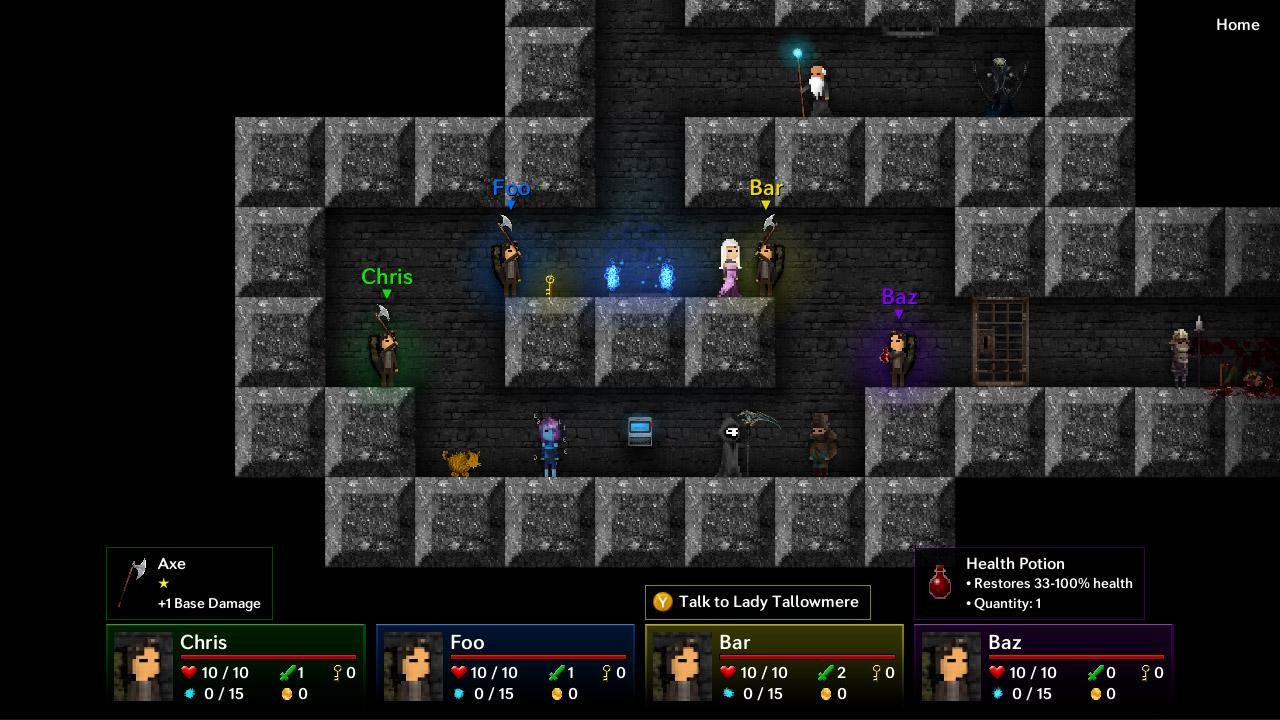
\includegraphics[width=1\textwidth]{StateOfTheArtScreenshots/tallowmere}
    \label{StateOfTheArt_Screenshots_Tallowmere}
    \caption{Screenshot of the game Tallowmere \cite{TallowmereScreenshot}}
\end{figure}

A 2D action platformer with an emphasis on executing your hero's jumping, shield-blocking, and weapon-attacking at the right moments as you move through a procedurally-generated dungeon. The game is available for:

\emph{Windows XP SP2 or newer, macOS 10.8 or newer, SteamOS, Ubuntu 12.04, Android 4.4 or newer, iOS 8.1 or newer, Wii U}

Features:

\begin{itemize}
    \item Randomly-generated rooms, with each room bigger than the last
    \item Blood splats, particle effects and sounds
    \item Skill-based gameplay, with no ammo, mana, or stamina gauges
    \item Traps and obstacles to dodge and avoid
    \item Special boss and event rooms
    \item Different weapons, shields and garments the hero can equip
    \item Infinite jumping
    \item Single Player and local co-op (up to 4 players)
    \item Permanent death, with a typical run lasting from 1 minute to 2 hours depending on skill
\end{itemize}

%------------------------------------------------

\subsection{Cave Story Plus}

\begin{figure}[ht]
    \center
    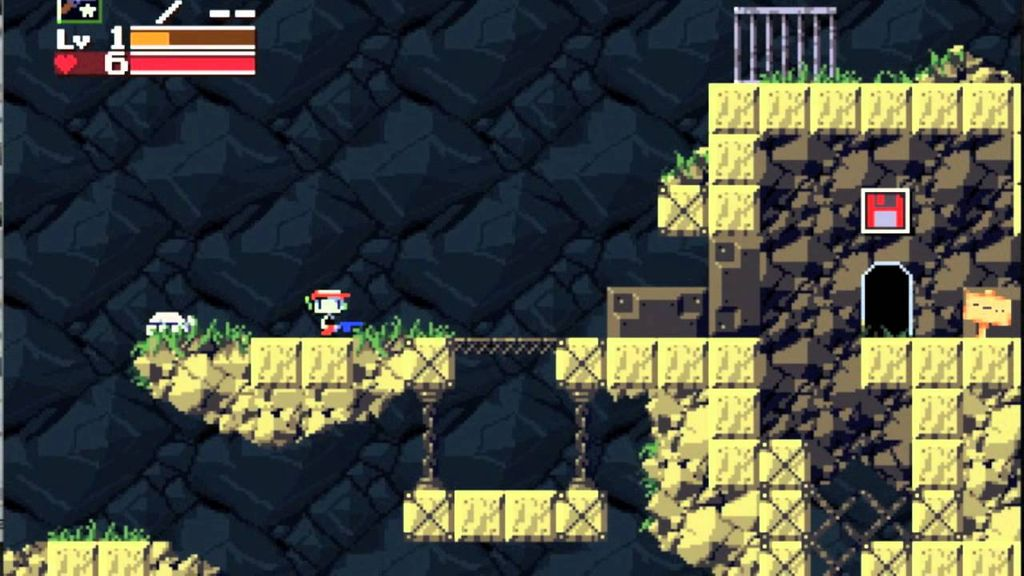
\includegraphics[width=1\textwidth]{StateOfTheArtScreenshots/cave_story_plus}
    \label{StateOfTheArt_Screenshots_CaveStoryPlus}
    \caption{Screenshot of the game Cave Story+ \cite{CaveStoryPlusScreenshot}}
\end{figure}

Cave Story+ is a Cave Story remake for PC, Mac and Nintendo Switch developed by Nicalis. It was released on Steam on November 22, 2011. The game features remastered graphics and music as well as several new game modes, of which one is only made exclusively to the Nintendo Switch version \cite{CaveStoryPlusWiki}.

Cave story+ has a selection of three difficulty levels; easy, standard and hard. Easy mode halves the HP of enemies and halves the damage they do to Quote (the main protagonist of Cave Story). The standard difficulty, is identical to the original game, in which Quote takes 100\% damage, and enemies have 100\% HP. Hard mode doubles the HP of enemies and removes all Life Capsules but one from the game, leaving the player with a maximum of 8 HP. Moreover, the Missile Launcher isn't available in the Hard mode.

Features:

\begin{itemize}
    \item Background music
    \item Over 20 boss battle games
    \item A variety of weaponry
    \item Four different game endings
    \item Hard mode for veterans
    \item Multiple versions available
    \item Metroid inspired setting
    \item Simple storyline
\end{itemize}

%------------------------------------------------

\subsection{Stardew Valley}

\begin{figure}[ht]
    \center
    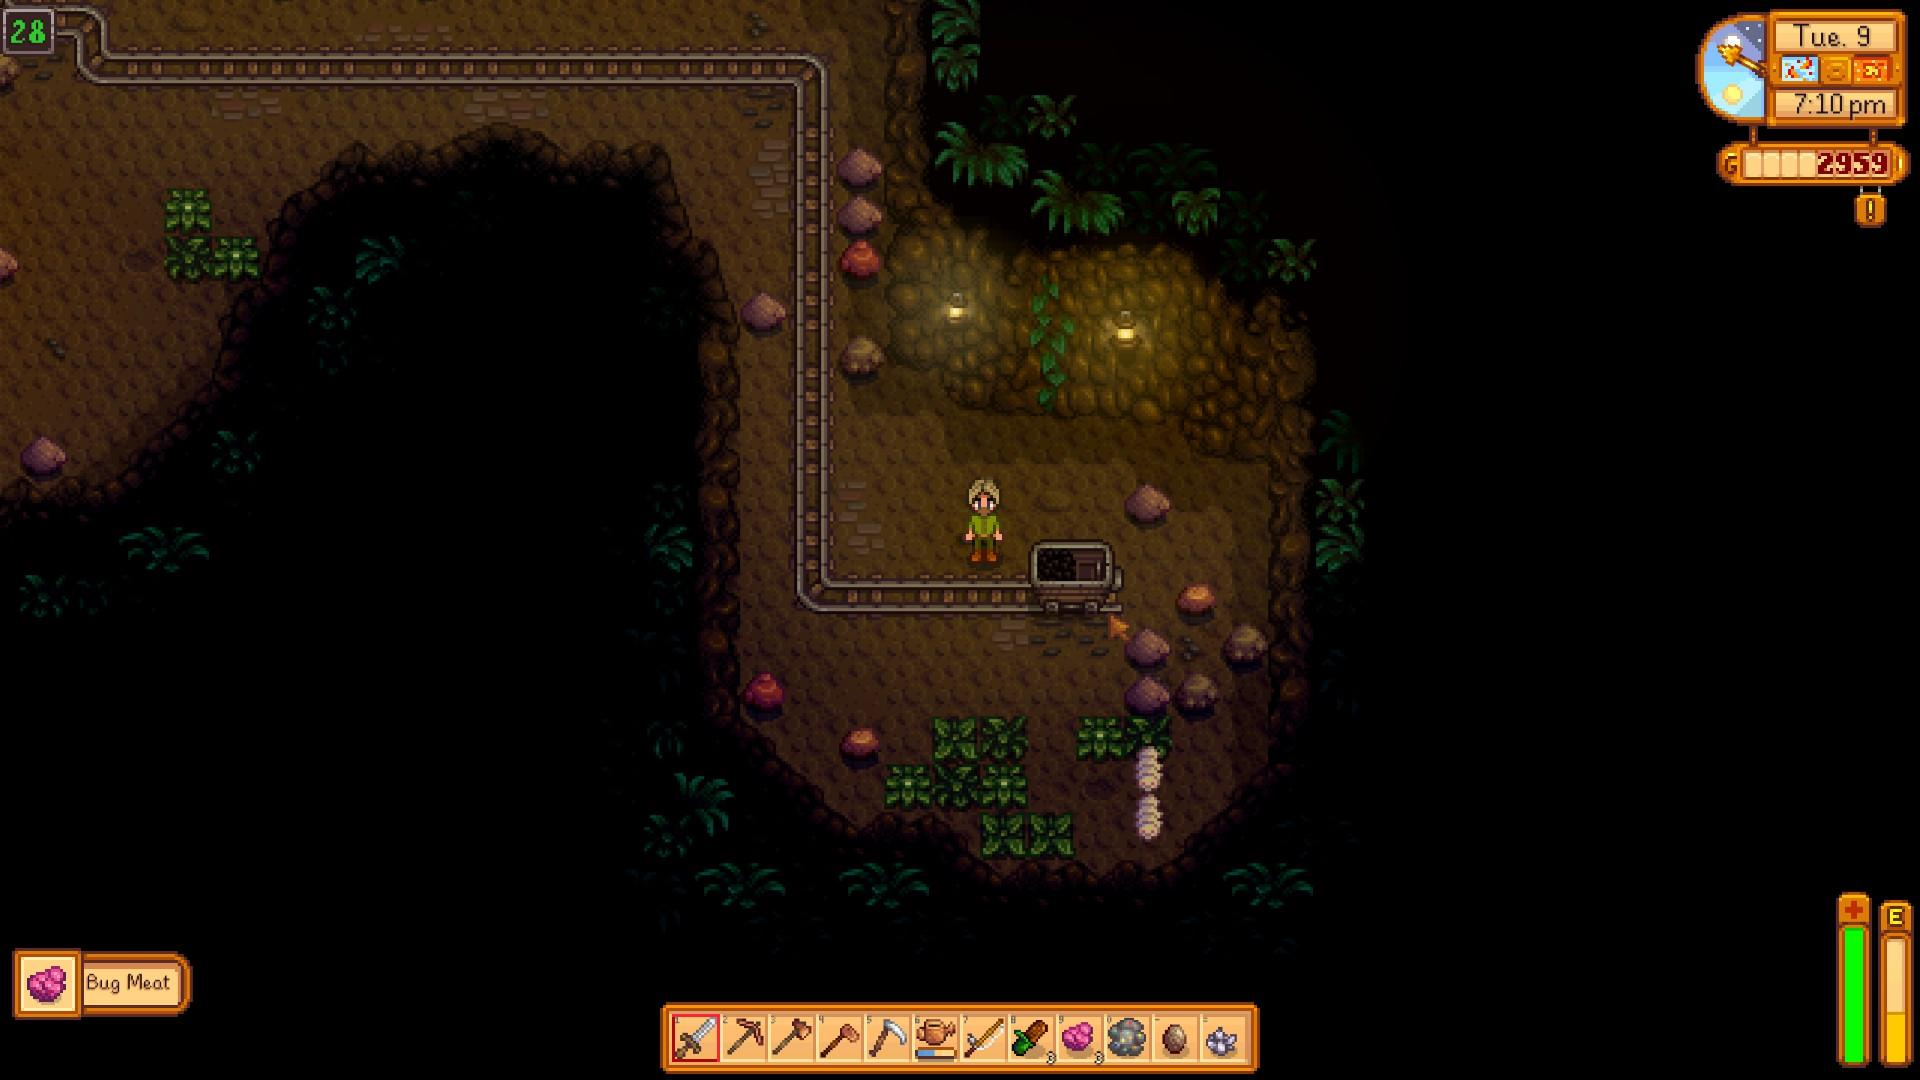
\includegraphics[width=1\textwidth]{StateOfTheArtScreenshots/stardew_valley}
    \label{StateOfTheArt_Screenshots_StardewValley}
    \caption{Screenshot of the game Stardew Valley \cite{StardewValleyScreenshot}}
\end{figure}

Stardew Valley is a 2D top-down indie farming simulation, which features an endless mine, where the player can fight, gather resources for the character and his farm and explore the different levels. The mines consist of an endless amount of procedurally generated levels, with checkpoints after every five levels. These checkpoints can be reached by an elevator on the first level in the mines. Each level consists of several elements, which are mainly gatherable stones and enemies, and also enemies. Furthermore, some levels have special elements, which are quicksand, minecarts, chests, and more. To reach the next level, the player has to find a ladder down, which can be found under a random stone or ore. They can either be destroyed by a pickaxe or bomb. This mine system is only a small part of the overall game but offers a fun and highly replayable experience due to the infinite amounts of levels.

Features:

\begin{itemize}
    \item Top-down rather than a sidescrolling game
    \item Procedurally generated levels
    \item Different themes and enemies for different level regions
    \item Inventory system
    \item Health and energy system
    \item Upgrading of weapons and armor
    \item Resource gathering (for overall game)
    \item Simple 8-bit graphics with customizable character
\end{itemize}

%------------------------------------------------

\subsection{Rogue Legacy}

\begin{figure}[ht]
    \center
    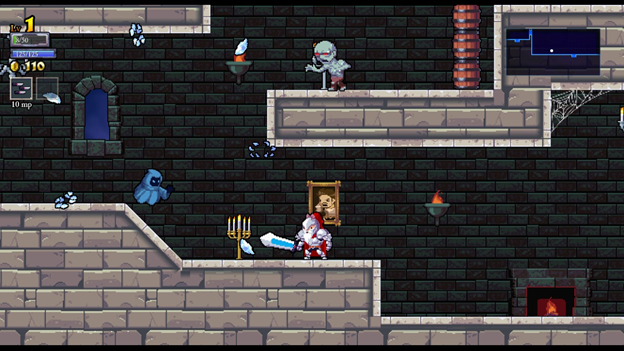
\includegraphics[width=1\textwidth]{StateOfTheArtScreenshots/rogue_legacy}
    \label{StateOfTheArt_Screenshots_RogueLegacy}
    \caption{Screenshot of the game Rogue Legacy \cite{RogueLegacyScreenshot}}
\end{figure}

Rogue Legacy is a 2D game, which was released in 2013 developed by Cellar Door Games. The game has been released for different platforms such as Microsoft Windows, Linux, OS X, PlayStation 3, PlayStation 4, PlayStation Vita and Xbox One \cite{RogueLegacyWiki}. The game is about exploring a randomly generated dungeon and collecting gold. The player(character) has default abilities such as jump and slash with a sword and secondary abilities such as magic attacks by using mana. The player has to defeat a boss in order to go to the next level \cite{RogueLegacyReview}.

Features: \cite{RogueLegacySteam}

\begin{itemize}
    \item Single player
    \item With sword, mana and life gauge to worry about
    \item Traps and obstacles to dodge and avoid
    \item More than 8 classes to choose from
    \item Over 60 different enemies
    \item Powerful weaponry and armor
    \item Tons of secret areas
    \item Boss in every stage
    \item Jump, run and dash
\end{itemize}

%------------------------------------------------

\subsection{Mega Miner}

\begin{figure}[ht]
    \center
    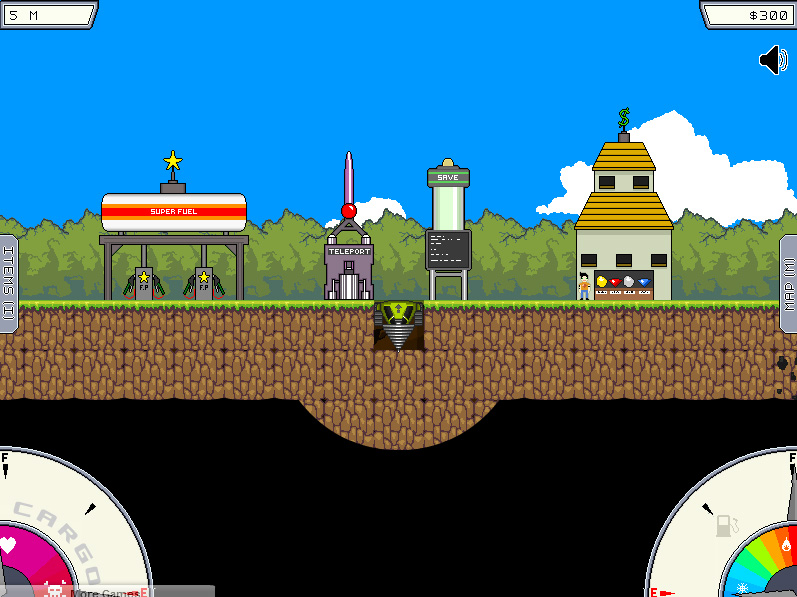
\includegraphics[width=0.8\textwidth]{StateOfTheArtScreenshots/mega_miner}
    \label{StateOfTheArt_Screenshots_MegaMiner}
    \caption{Screenshot of the game Mega Miner \cite{MegaMinerScreenshot}}
\end{figure}

Mega miner is a 2D game developed by Armor Games. The main task in the game is to drill a mine and while this process collects gold, silver, coal and other minerals. Then the player (character) can sell it for cash and upgrade his mining machine by new coolers etc. This game is qualified as a strategy game.

Features:

\begin{itemize}
    \item Single player
    \item Gold, silver, coal and other minerals to collect
    \item Rocks as obstacles to avoid
    \item One map
    \item No enemies
    \item Possibility to upgrade character (drill)
\end{itemize}

%------------------------------------------------

\subsection{Spelunky}

\begin{figure}[ht]
    \center
    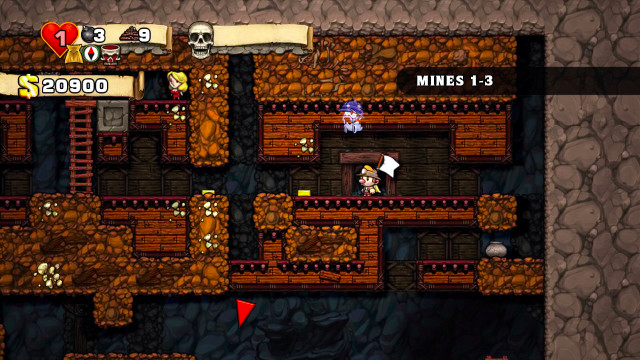
\includegraphics[width=1\textwidth]{StateOfTheArtScreenshots/spelunky}
    \label{StateOfTheArt_Screenshots_Spelunky}
    \caption{Screenshot of the game Spelunky \cite{SpelunkyScreenshot}}
\end{figure}

Spelunky is a 2D cave exploration/treasure-hunting game inspired by classic platform games such as Rayman, Super Mario, and Sonic the Hedgehog. One of the crucial features that differentiate this game to the classic versions, is that the game is top-down rather than sidescrolling, which leaves the player with a completely different feel. With an inventory full of bombs, ropes, and your own whip, the aim is to creatively maneuver through the fully-destructible ancient caves. In order to complete levels, you have to search deep in the underground for a door, while encountering a variety of enemies, as well as traps and treasure. It's a challenging game that will likely test your patience since you will die continuously. But with many deaths comes experience, and eventually, as you beat the level, the frustration is overtaken by a great feeling of satisfaction.

\textbf{Pros and Cons:}

\textbf{Pro:} Skill based gameplay. \emph{In Spelunky the player has everything needed from the start so it is only the skill level of the player that determines whether you advance or not.}

\textbf{Pro:} Roguelike genre allow for quick sessions. \emph{Since the gameplay is so quick, the player will die quite often which means that the sessions tend to be quite short. This makes for a game that can be played in quick bursts throughout the day.}

\textbf{Con:} No check-point system. \emph{You can't save the game and you can't go back to a level with your previous equipment.}

\textbf{Con:} Hard to master. \emph{The game is difficult to the point of frustration.}

Features:

\begin{itemize}
    \item Top-down rather than a sidescrolling game
    \item Skill-based gameplay
    \item Single player and local co-op (up to 4 players)
    \item Traps and enemies to dodge and avoid
    \item Inventory system primarily with bombs and ropes
    \item Money collecting for the shopkeeper in-between levels
    \item Full maneuverability with infinite jumping and running
\end{itemize}

%------------------------------------------------

\subsection{Nuclear Throne}

%------------------------------------------------

\subsection{Conclusion}
Conclusion.

%----------------------------------------------------------------------------------------
%	MARKET ANALYSIS
%----------------------------------------------------------------------------------------

\newpage
\section{Market analysis} \label{MarketAnalysis}

%----------------------------------------------------------------------------------------
%	DOCUMENTATION
%----------------------------------------------------------------------------------------

\newpage
\section{Documentation}

\subsection{Choosing the game engine}

Deciding on a game engine is not an easy task, especially for Java. In the group, we split up the research of individual game engines, so that we can gather information about as many as possible before deciding on one. The procedure of finding relevant frameworks and game engines was fairly easy, by searching on a list of game engines on Wikipedia \cite{ListOfGameEngines}, using Google search and reading through forums to determine the public opinion on this topic. It quickly became apparent, that the market is rather thin when it comes to Java-based game engines, the big players like Unity and Unreal Engine rely on \texttt{C} variations.

We researched the option of using a native Java library like \texttt{JavaFX}, and therefore having to write a lot of basic code ourselves. The group decided against this option by a majority vote. Not having to deal with a lot of very basic problems and therefore being able to develop the game farther and with more features, was more appealing to the majority of the group members.

Moving on, the group settled on a couple of game engines or frameworks to research: \texttt{libGDX, LWJGL, jMonkeyEngine, mini2Dx} and \texttt{Slick2D}. This selection is mostly by scavenging forum posts and the first page of Google for the search of "Java Game Engines". One particular Reddit post \cite{RedditJavaGameEngines} named all of them.

Since \texttt{libGDX} is based on \texttt{LWJGL}, it is easy to compare them. \texttt{LWJGL} is very low-level and doesn't provide many features, compared to \texttt{libGDX}. It is also harder to start off with as a beginner in programming \cite{StackExchangeLibGDXLWJGL}, which is why we went with \texttt{libGDX}. Furthermore, the \texttt{jMonkeyEngine} is mainly developed for 3D applications, which rules it out for our project. \texttt{Mini2Dx} and \texttt{Slick2D} are both based on \texttt{LWJGL} too, but we already decided in favour of \texttt{libGDX}, since we had a working demo running and an overall good feeling with it. It is also important to note, that both of those have a smaller community and therefore documentation, which is also a reason, why the group decided to stick with the "big guy". 

\subsection{libGDX Setup}

To setup a libGDX project in IntelliJ IDEA, the official setup tool (see Figure \ref{fig:LibGDXSetupScreenshot}) needs to be used. This creates a Gradle project with all necessary files, adds optional extensions by default and defines the deployment platforms (Desktop, Android, iOS and HTML). By clicking on \emph{Advanced} and selecting IntelliJ IDEA or a different IDE, this tool also creates the project files for the specific IDE.

\begin{figure}[h]
    \centering
    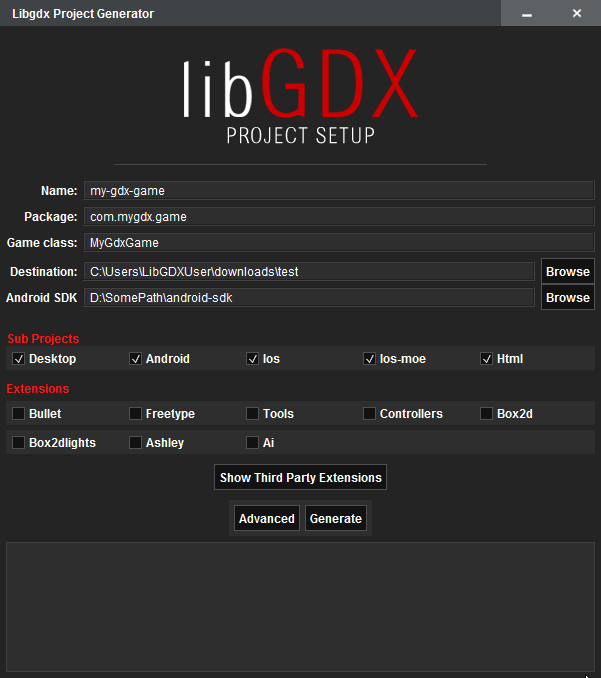
\includegraphics[width=0.6\textwidth]{libGDX_setup.png}
    \caption{libGDX Setup Tool}
    \label{fig:LibGDXSetupScreenshot}
\end{figure}

The import into IntelliJ is easy, just open the project and an import pop-up appears. By simply clicking \texttt{Ok}, everything will be imported and set up and the project is ready. To run the application in an desktop environment, the build configuration needs to be updated first, by setting the working directory to the \texttt{assets} folder of the project. With this being done, the set-up is complete.

\subsection{Using key bindings for player input}

Key bindings in games are used to give the players the possibility to individually adjust their setup as they like. Players might want to change the assigned keys for certain actions in the game, if they have unusual keyboard layouts, use other types of input devices like gamepads, or simply like to change a certain key. This gives more flexibility since hard-coded keys can cause frustration and cause an unfavourable opinion about the game.

LibGDX has two different kinds of input processing, the first one being the \texttt{Input} class included in the framework, which uses polling to get key presses. The second method is using an \texttt{InputProcessor}, also included in the framework, which uses events to control input. The key difference between those is, that one can check if a specific key is being pressed at the time of checking with the polling method. An input processor, however, triggers events when certain input events happen, like pressing down a key and then delivering the key code of the pressed key. This allows the input management to be more "clean" and efficient since one can't easily check if one of many flexible keys is being pressed without an input processor.

In order to change and save key bindings, there needs to be a data structure. This is represented in the \texttt{KeyBindingObject} class (see \ref{KeyBindingObject.java}). One object each represents a single action in the game, represented by a String, and an array of integers, which represent the codes of the keys that are assigned to this action. Therefore, multiple keys can be assigned to one action.

Furthermore, the game has to save this information in a file to make it persistent, or the information will be lost once the application is closed. Therefore, the game will save and load the key bindings into a JSON (JavaScript Object Notation) file, which is a standard data interchange format. Handling this operation is done by the \texttt{KeyBindings} class (see \ref{KeyBindings.java}) class. 

This class has public lists of the type Integer, which store the key codes for each individual action. These lists are read by the game to process input. In the constructor of the class, the program searches for the JSON file and if it exists, it reads it with the help of \texttt{GSON} \cite{GSON}, an open-source library by Google to convert Java Objects into JSON strings and back. If the file doesn't exist or is empty, a new one will be created and the default keys will be assigned to each action by writing them to the new file and then read them again. Those default keys are hardcoded in the constructor as a \texttt{KeyBindingObject} array.

However, if the file does exist, the JSON string is read from it and converted to an array of \texttt{KeyBindingObject}'s. Each key object will then be assigned to the proper list, that was mentioned earlier. This is done by looping through each object and adding it to the lists by comparing the String attribute, described as \texttt{}{action}. This procedure is called deserialization and can be seen in \ref{KeyBindings.java} in the \texttt{deserializeKeyBindings()} method.

An exemplary key bindings JSON key binding file looks like this:
\inputminted[linenos,breaklines]{json}{code/json/keybindings.json}

An array in JSON starts with a \texttt{[}, hence the bracket at the start and end. The \texttt{KeyBindingObject}'s in between are items of that array. Each item has a String identifier and another array for the corresponding key codes. JSON separates key and value with a \texttt{:} symbol.

As described earlier, the game uses a \texttt{InputProcessor} to handle gameplay relevant input. Since the game has to recognize when a key is pressed, and not just fire an event once a key is pressed down once, it uses public booleans to toggle between an action being active or not. Otherwise, the player would get a move impulse, for example, only once instead of for the duration of the key press. This logic is located in the \texttt{GameplayInputProcessor} class (see \ref{GameplayInputProcessor.java}). When a key is being pressed down or being released, it checks, if the key code of the pressed key is in one of the lists. If that is the case, the \texttt{boolean} is toggled. This \texttt{boolean} is a member of the \texttt{PlayScreen} class and is \texttt{public static} to be available in this class, and is being imported in a static context, hence the missing class reference in the Input Processor class.

Finally, all of this is then used in the \texttt{update} loop of the \texttt{PlayScreen}, which is executed each frame. This is an example of the movement in the right direction:

\begin{minted}[linenos,breaklines]{java}
if (isPressingMoveRight &&
    player.body.getLinearVelocity().x <= player.getMaxWalkVelocity()) 
{
    player.body.applyLinearImpulse(new Vector2(player.getWalkImpulseVelocity(), 0), player.body.getWorldCenter(), true);
}
\end{minted}

Here, it is simply being checked, if the user presses a key that is associated with the action of moving in the right direction, by evaluating \texttt{isPressingMoveRight}.

\subsection{Visual Documentation}

\subsection{Tech Documentation}

\subsection{Animations}

\subsection{Collision detection}

\subsection{Item collecting}

\subsection{Player and enemy health management}

\subsection{Sprites}

\subsection{Maps}

%----------------------------------------------------------------------------------------
%	DISCUSSION
%----------------------------------------------------------------------------------------

\newpage
\section{Discussion}

Discussion.

%----------------------------------------------------------------------------------------
%	CONCLUSION
%----------------------------------------------------------------------------------------

\newpage
\section{Conclusion}

Project Conclusion.

%----------------------------------------------------------------------------------------
%	BIBLIOGRAPHY
%----------------------------------------------------------------------------------------

\newpage
\printbibliography[heading=bibintoc,title={References}]

%----------------------------------------------------------------------------------------
%	APPENDIX
%----------------------------------------------------------------------------------------

\newpage
\appendix
\section{Source Code Appendix}

\subsection{MainGameClass} \label{MainGameClass.java}
\inputminted[linenos,breaklines]{java}{code/MainGameClass.java}

\subsection{GameProgress}

\subsection{Input}
\subsubsection{GameplayInputProcessor} \label{GameplayInputProcessor.java}
\inputminted[linenos,breaklines]{java}{code/Input/GameplayInputProcessor.java}

\subsection{Items}

\subsection{KeyBindings}
\subsubsection{KeyBindingObject} \label{KeyBindingObject.java}
\inputminted[linenos,breaklines]{java}{code/KeyBindings/KeyBindingObject.java}
\subsubsection{KeyBindings} \label{KeyBindings.java}
\inputminted[linenos,breaklines]{java}{code/KeyBindings/KeyBindings.java}

\subsection{Scenes}

\subsection{Screens}
\subsubsection{PlayScreen} \label{PlayScreen.java}
\inputminted[linenos,breaklines]{java}{code/Screens/PlayScreen.java}

\subsection{Sprites}

\subsection{Statistics}

\subsection{Tools}

\subsection{Widgets}

%------------------------------------------------
\end{document}